\section{Distribuições Probabilísticas}
%--- Distributions ----------------------------------------------------%

\tikzset{
    declare function={
      gaussian(\m,\s)=1/(\s*sqrt(2*pi))*exp(-((x-\m)^2)/(2*\s^2));%
      binomial(\n,\p)=\n!/(x!*(\n-x)!)*\p^x*(1-\p)^(\n-\x);%
      poisson(\l)=(\l^{x})*exp(-\l)/({x}!);%
    }
}

%--- Slide 1 ----------------------------------------------------------%

\subsection{Distribuições Discretas}
\subsubsection{Binomial}
\begin{frame}{Binomial}
  \centering
  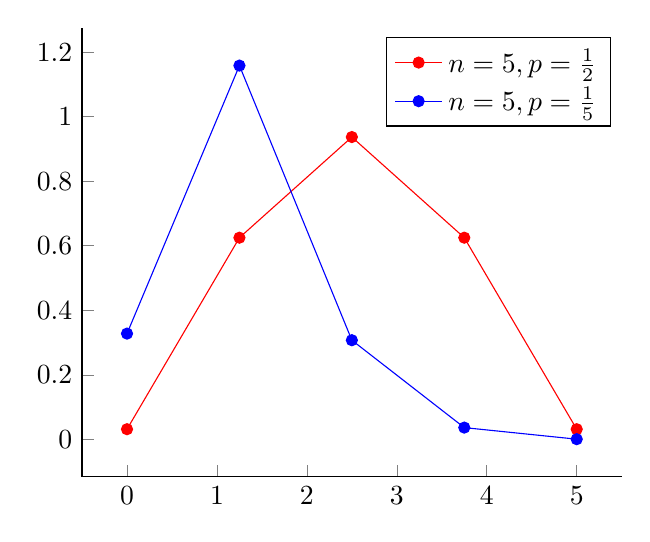
\begin{tikzpicture}[mark=*]
      \begin{axis}[every axis plot post/.append style={
          domain=0:5, samples=5}, % All plots: from 0:5, 5 samples only
          axis x line*=bottom, % no box around the plot, only x and y axis
          axis y line*=left, % the * suppresses the arrow tips
          enlarge x limits=true,
          ] % extend the axes a bit

          \addplot [red] {binomial(5, 0.5)};
          \addlegendentry{$n=5, p=\frac{1}{2}$}
          \addplot [blue] {binomial(5, 0.2)};
          \addlegendentry{$n=5, p=\frac{1}{5}$}
      \end{axis}
  \end{tikzpicture}
\end{frame}

%--- Slide 2 ----------------------------------------------------------%

\subsection{Distribuições Contínuas}
\subsubsection{Normal}
\begin{frame}{Normal}
    \centering
    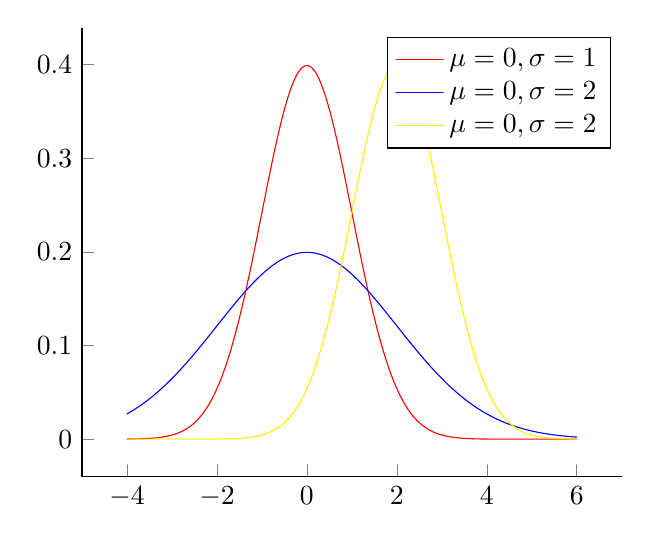
\begin{tikzpicture}[line cap=round]
        \begin{axis}[every axis plot post/.append style={
            mark=none,domain=-4:6,samples=200,smooth}, % All plots: from -4:4, 200 samples, smooth, no marks
            axis x line*=bottom, % no box around the plot, only x and y axis
            axis y line*=left, % the * suppresses the arrow tips
            enlarge x limits=true,
            ] % extend the axes a bit

            \addplot [red] {gaussian(0, 1)};
            \addlegendentry{$\mu=0, \sigma=1$}
            \addplot [blue] {gaussian(0, 2)};
            \addlegendentry{$\mu=0, \sigma=2$}
            \addplot [yellow] {gaussian(2, 1)};
            \addlegendentry{$\mu=0, \sigma=2$}
        \end{axis}
    \end{tikzpicture}
\end{frame}
